\begin{figure}[htbp]
    \centering
    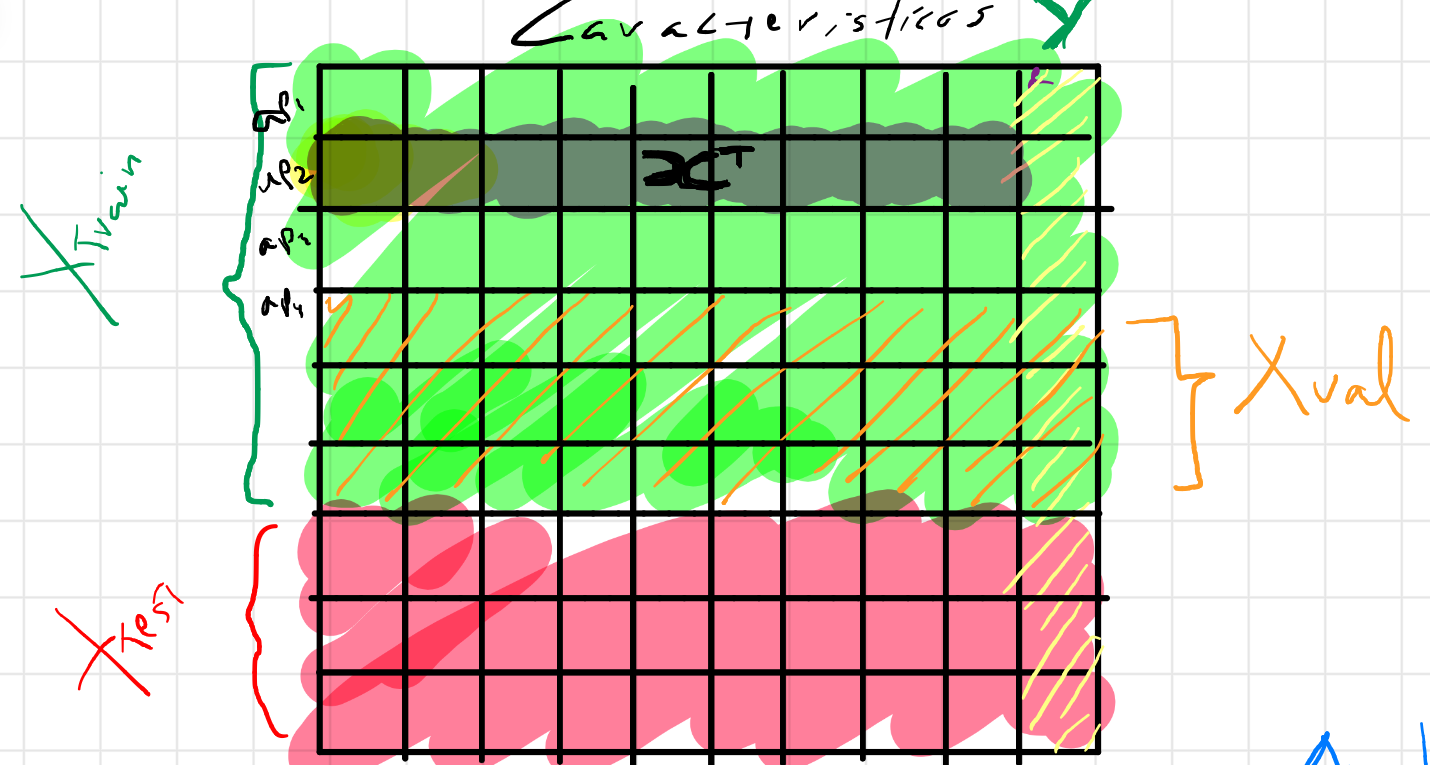
\includegraphics[width=0.8\linewidth]{Parts/LearningProblem/Chapters/LearningProblemConcepts/Images/XtrainXtestXval.png}
    \caption{}
    \label{fig:Xtrain-Xval-Xtest}
\end{figure}

Coluna Y são os preços de apartamentos, as outras são características dos apartamentos, m², número de quartos e entre outros.


\begin{equation*}
    \mathbf{f} = \{ f_{\theta} \mid \theta \in \mathcolor{Blue}{\Theta} \}
\end{equation*}

\begin{figure}[htbp]
    \centering
    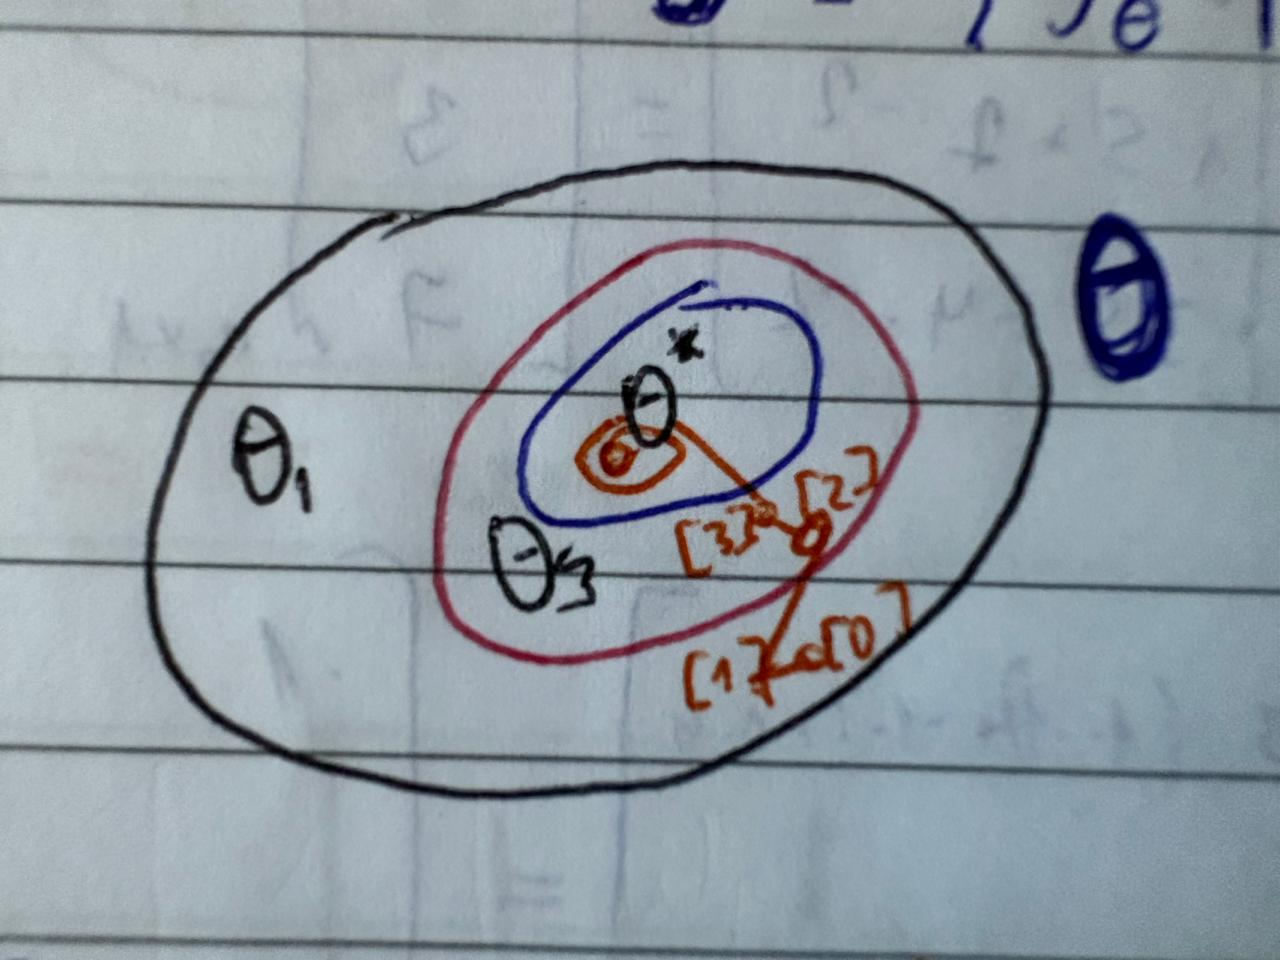
\includegraphics[width=0.4\linewidth]{Images/Aula 2/thetaFunction.jpeg}
    \caption{}
    \label{fig:thetaFunction}
\end{figure}

\begin{equation*}
    \mathbf{f_{\theta}} : \mathbb{R}^{\mathcolor{orange}{D}} \rightarrow \mathbb{R}^{\mathcolor{orange}{1}} \\
\end{equation*}

\begin{equation*}
    \{\mathbf{x^T} | \mathbf{x^T} \in \mathbb{R}^{1 \times \mathcolor{orange}{D}} \} \rightarrow  \{\mathcolor{ForestGreen}{y} \in \mathbb{R}^{1 \times 1}\}
\end{equation*}


\begin{figure}[htbp]
    \centering
    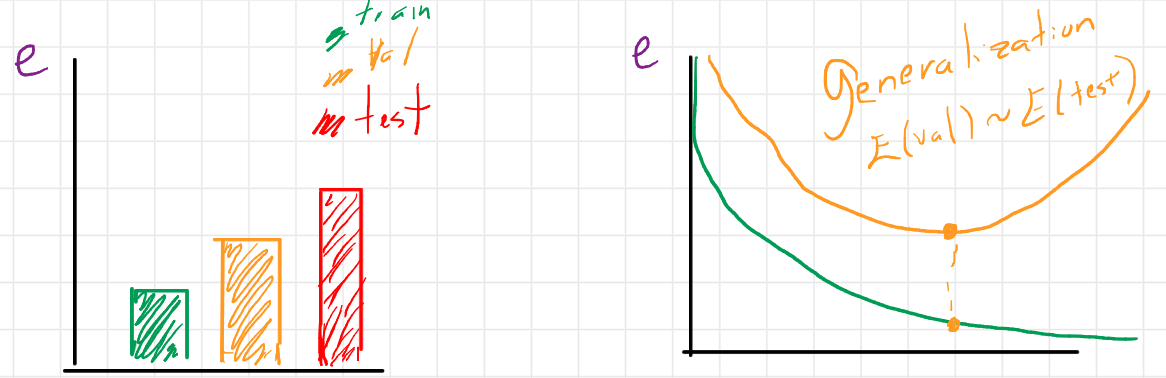
\includegraphics[width=0.8\linewidth]{Parts/LearningProblem/Chapters/LearningProblemConcepts/Images/erroXtrainXtest.png}
    \caption{}
    \label{fig:Xtrain-Xval-Xtest}
\end{figure}


\begin{equation*}
    \mathcolor{ForestGreen}{y} = X{\mathcolor{orange}{w}} \quad ; 
    \mathcolor{ForestGreen}{y} = 
    \begin{bmatrix}
    \,|\, & \,|\, &        & \,|\, \\
    \mathbf{x}_{\mathcolor{Orange}{1}} 
        & \mathbf{x}_{\mathcolor{Orange}{2}}
        & \cdots 
        & \mathbf{x}_{\mathcolor{Orange}{D}} \\
    \,|\, & \,|\, &        & \,|\, \\
\end{bmatrix}_{\mathcolor{ForestGreen}{N}\times\mathcolor{orange}{D}} \times
\begin{bmatrix}
    \mathcolor{orange}{w}_{\mathcolor{orange}{0}} \\
    \mathcolor{orange}{w}_{\mathcolor{orange}{1}} \\
    \vdots \\
    \mathcolor{orange}{w}_{\mathcolor{orange}{d}}
\end{bmatrix}_{\mathcolor{orange}{D}\times 1}
\end{equation*}

Vamos continuar pensando que a matriz $X$  onde cada linha é um apartamento e cada coluna é alguma informação do apartamento. Logo, estamos querendo saber o preço desses apartamentos a partir das informações, será que apartamentos com mais quarto são mais caros por exemplo. Então temos que o $\mathcolor{orange}{w}$ é um vetor coluna de pesos, pense que cada informação do apartamento tem um peso associado a ele que vai ser importante para o cálculo do preço final. Então $\mathcolor{ForestGreen}{y}$ é um vetor coluna que contém os preços de todos os apartamentos.